\chapter{气体电离探测器}
将被测射线转换为可观测信号的特殊器件,称为电离辐射探测器,简称探测器。
探测器形成信号需要3步:
\begin{compactenum}
	\item 辐射粒子射入“灵敏体积”(立体角);
	\item 入射粒子与灵敏体积内的工作介质相互作用,损失能量并形成电离或激发(本征探测效率);
	\item 探测器通过自身特有工作机制将入射粒子的电离或激发效果转化为某种输出信号(分辨率)。
\end{compactenum}

各种探测器关注的核心问题是载流子,按探测介质和作用机制,探测器可分为三类:
\begin{compactitem}
	\item 气体电离探测器:电子-离子对;
	\item 闪烁体探测器:第一打拿极(dynode)收集到的光电子;
	\item 半导体探测器:电子-空穴对;
\end{compactitem}
气体探测器是以气体为工作介质,由射线在其中产生电离效应引起输出电信号的探测器。
按照产生信号的工作机制,可分为:电离室、正比计数器、G-M计数器以及自熄流光管SQS计数器等。

\section{气体中离子与电子的运动规律}

气体本来是绝缘的,有了电子-离子对这个载流子就能导电了。
\paragraph{气体的电离与激发}
入射的带电粒子会引起气体分子的电离和激发,同时损失能量。%ns时间后,带电粒子停止了,成为中性原子,但是在探测器内留下了很多电子-离子对。

\textbf{平均电离能}$W$:带电粒子在气体中产生一个电子-离子对所需的平均能量。故产生的平均电子-离子对的数目为
\begin{align}
	\avg N=\frac{E_0}W.
\end{align}
重要特性:同种气体的平均电离能基本是个常数($W\sim\SI{30}{eV}$),从而
\[
	\avg N\propto E_0,
\]
可以根据载流子数目$N$来测量入射带电粒子的能量$E_0$。由于$N$服从Fano分布,我们希望载流子数目越多越好。



\paragraph{气体中离子、电子的运动}
电子和正离子在气体中运动,和气体分子不断地碰撞,有以下物理过程:
\subparagraph{扩散(diffusion)}
电子云随时间扩散为空间Gauss分布,扩散系数$D\,(\si{cm^2/s})$
\[
	D:=\frac13\avg v\lambda,
\]
电子的平均自由程$\lambda$和乱运动平均速度$\avg v$都比离子的大,故$D_\elc>D_\i$

扩散效应对电子的收集影响不大,但对电离产生位置信息的确定有一定影响($\sim\si{mm}$)。
\subparagraph{电荷转移效应(charge transfer)}
正离子与中性的气体分子碰撞时的电荷转移。\footnote{电荷转移效应在混合气体中较明显,如有机自熄G-M管中的$\nuc{Ar}^+(\SI{15.7}{eV})$和$\nuc{C_2H_5OH}(\SI{11.3}{eV})$,后者对于自熄起到了至关重要的作用。}

\subparagraph{吸附(electron attachment)}
电子与气体分子碰撞时被气体分子俘获,形成负离子。
\begin{definition}{吸附系数}{}
	吸附系数$p$:在与气体分子的每次碰撞中,电子被俘获%形成负离子
	的概率%称为该气体的吸附系数。
	\begin{compactitem}
		\item 非负电性气体($p<10^{-6}$):
		惰性气体、$\nuc H_2,\nuc N_2$、多原子分子气体。
		\item 负电性气体($p>10^{-5}$):
		$\nuc{O_2,H_2O}\enspace (\sim 10^{-4})$,卤素($\sim 10^{-3}$)。
	\end{compactitem}
\end{definition}
\subparagraph{复合(recombination)}
正负电荷可能复合成中性的原子或分子,有电子正离子复合、正负离子复合两种。

复合引起的离子对数目的损失率(\si{/cm^3.s}):
\[
	-\pv{n^+}t=-\pv{n^-}t=\alpha n^+n^-.
\]
$\alpha$为复合系数(\si{cm^3/s})。同种气体$\alpha_\elc\ll\alpha_\i$,

复合会导致载流子减少,从而信号幅度降低、统计性变差。%在探测器正常工作中应尽量避免
因此应选择吸附系数小的工作气体,杜绝负电性气体进入,保持纯度。
\begin{definition}{三种复合}{}
	\begin{compactitem}
		\item germinate (initial)复合
		\item columnar复合:同一电离径迹上。重离子、裂变碎片时严重;
		\item volume复合:发生在扩散、漂移时。计数率高的时候严重。
	\end{compactitem}
\end{definition}
\noindent
外加电场可以抑制germinate和volume复合,但columnar复合难以消除。

\paragraph{外加电场下离子、电子的运动}
离子和电子有两种运动:扩散和定向漂移。

\subparagraph{离子}
两次碰撞之间离子从电场获得的能量在碰撞中又会损失掉,因此离子的能量积累不起来,平均动能与没有电场的情况相似。

离子漂移速度
\begin{align}
	u^\pm=\mu^\pm\frac EP.
\end{align}
$E$为电场强度,$P$为气体压强,$\mu^\pm$为离子迁移率,仅与气体特性有关。
为求离子迁移率$\mu^\pm$,作三个假设:
\begin{compactenum}
	\item 离子在电场方向上的漂移速度$\ll$乱运动的速度。
	\item 两次碰撞间离子从电场所获能量在碰撞时全部传给了气体原子;
	\item 碰撞后离子的运动取向为各向同性,即漂移速度为0。
\end{compactenum}
离子的迁移率可表示为
\[
	\mu^\pm=\frac{e\lambda_0}{2M\avg v}.
\]
$\lambda_0$是离子在单位气压气体中的自由程,$\avg v$是乱运动的平均速度,离子的平均动能不随电场而变,故近似为常数,由温度决定。

\subparagraph{电子}电子与气体原子发生弹性碰撞时损失的能量很小,因此电子在两次碰撞中由外电场加速的能量可积累起来。平均动能与电场强度有关,则电子的迁移率$\mu$不是常数。漂移速度$u$与约化场强$E/P$不再成正比,一般给出的是实验曲线。

\subparagraph{电子与离子漂移的区别}
\begin{compactenum}
	\item 电子漂移速度$\sim\SI{e6}{cm/s}$,离子漂移速度$\sim\SI{e3}{cm/s}$。
	\item 电子的漂移速度对组成气体的组分极为敏感。
	
	在单原子分子气体中加入少量多原子分子气体(如CO$_2$、H$_2$O等)时,电子的漂移速度有很大的增加。
\end{compactenum}
\paragraph{气体放电}
\textbf{雪崩}(avalanche):电子在气体中的碰撞电离过程。

电离产生的电子能量较低($\delta$电子除外),无法再形成电离;
但是当存在外加电场时,电子将从电场中不断地获得能量;
随着电场强度$E$的增加,电子获得的能量也在增加,%电子温度提升,
直到弹性碰撞、激发、电离。
\subparagraph{发生雪崩的条件}
\begin{compactenum}
	\item 强电场:$\SI{1}{atm}$下发生雪崩的阈值电场$E_\thres\sim\SI{e6}{V/m}$;
	\item 自由电子:
	\begin{compactenum}
		\item 电离产生的电子;
		\item 雪崩后退激光子和器壁作用,打出光电子引发新的雪崩;
		\item 雪崩正离子可能在器壁上打出二次电子引发新的雪崩。
	\end{compactenum}
\end{compactenum}
气体放电方式:
\begin{compactitem}
	\item 非自持放电:雪崩从产生到结束,只发生一次。
	\item 自持放电;通过光子的作用和二次电子发射,雪崩持续发展。
\end{compactitem}
\paragraph{小结}气体中离子和电子的运动。无外加电场时,载流子经过扩散、电子复合、吸附、离子复合,数量减少,统计性变差。所以\textbf{外加电场抑制复合}是必要的。

若电场再增强,就会发生雪崩。虽然雪崩过程让载流子数量增多了,但并不会带来统计性的改善。一是倍增同一个常数并不会改变相对偏差,二是倍增常数也是随机的。事实上,作为级联变量,
\[
	\nu_\xi^2=\frac FN+\frac1N\nu_M^2>\frac FN.
\]
因此雪崩带来的$\nu_M$会增大$\nu_\xi$。若电场再增强,光电子和二次电子使$N$再增加,就会偏离正比关系。
\newpage
\begin{center}
	\captionof{table}{气体探测器工作区}
	\begin{tabular}{ccl}
		\toprule
		复合区&&复合效应导致载流子减少\\
		饱和区&\checkmark&复合被抑制,载流子产生饱和\\
		正比区&\checkmark&开始产生雪崩效应,倍增系数与电场有关\\
		有限正比区&&弱电离、强电离粒子的离子鞘使得等效电场下降\\
		G-M工作区&\checkmark&最终电离效果、总载流子数量与原始电离没有关系\\
		连续放电区\\
		\bottomrule
	\end{tabular}
\end{center}

\section{电离室的工作机制和输出回路}

\paragraph{电离室的基本结构}
电离室虽然结构有多种形式,但基本结构相同。由高压极(K)、收集极(C)、保护极(G)\footnote{
	保护极的作用:
	\begin{compactenum}
		\item 使灵敏体积边缘处的电场保持均匀;
		\item 防止大高压时有漏电流从负载电阻$R_L$流过,产生噪声。
	\end{compactenum}
}
和负载电阻($R_L$)。典型结构有平板型和圆柱型。



灵敏体积:由通过收集极边缘的电力线所包围的两电极间的区域。
\paragraph{工作气体}
充满电离室内部空间,是电离室的工作介质。
应选用电子吸附系数$p_\elc$小的气体(如Ar中加少量多原子分子气体CH$_4$)。

气压$\SIrange{0.1}{10}{\atm}$。为了保证气体的成分和压力,一般电离室均需要一个密封外壳将电极系统包起来。
但也可以是流气的。
\paragraph{输出信号产生的物理过程}
以气体探测器的简化结构入手,极板a上加高压$V_0$,极板a, b间电容量为$C_1$,则两极板的电荷量$Q_0=C_1V_0$
\usetikzlibrary {circuits.ee.IEC}
\begin{center}
	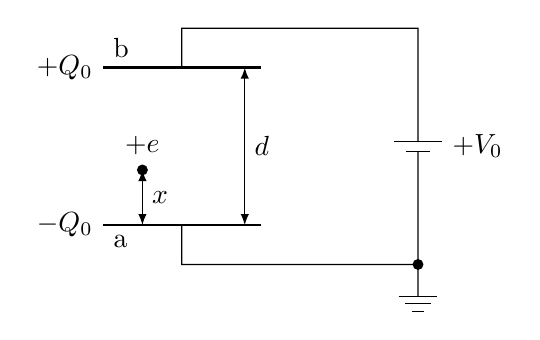
\begin{tikzpicture}[circuit ee IEC]
		\draw [thick] (-4, 2.5) node [left] {$+Q_0$} node [above right] {b} -- (-2, 2.5);
		\draw [thick] (-4, .5) node [left] {$-Q_0$} node [below right] {a} -- (-2, .5);
		\draw [latex-latex] (-2.2, .5) -- (-2.2, 2.5) node [midway, right] {$d$};
		\draw [latex-latex] (-3.5, .5) -- (-3.5, 1.2) node [midway, right] {$x$} node [contact={info={$+e$}}] {};
		\draw (-3, .5) to (-3, 0) to (0, 0) to [ground={at end}] (0, -.5);
		\draw (-3, 2.5) to (-3, 3) to (0, 3) to [battery={info={$+V_0$}}] (0, 0) node [contact] {};
	\end{tikzpicture}
	\captionof{figure}{气体探测器简化结构}
\end{center}
在电离室内某点引入一单位正电荷$+e$,它将在两极板上分别感应出
一定的负电荷$-q_+,-q_-$,由Ostrovski-Gauss定理  %ОсmроTраgсkuй-Gauß定理
\[
	\begin{cases}
		q_+=e\,\frac xd;\\
		q_-=e\kh{1-\frac xd}.
	\end{cases}
\]
当$+e$电荷沿电场向收集极b运动,$q_+$减少,$q_-$增加。这就相当于感应电荷从外回路流过,即在外回路流过电流$i^+(t)$。
当$+e$到达b极板中和。外回路电流结束,流过外回路的总电荷量为  $q_+$;同理,$-e$漂移引起正感应电荷在回路中流过的电荷量为$q_-$,外回路流过电流$i^-(t)$与$i^+(t)$方向相同。
\subparagraph{结论}
射线电离产生电子-离子对,来自于同一个中性原子(分子),\textit{产生于同一位置},故任何一对载流子在完成漂移后,外电路流过的电荷量为$e$,与其产生位置无关。
灵敏体积内产生的$N_0$对载流子在完成漂移后,外电路流过的电荷量为$N_0e$。

电子速度$\gg$离子速度,故电子先被收集,此后外回路中只有正电荷的感应电流,最后外回路感应电流消失。
\paragraph{电离室的输出回路}
输出回路是信号电流流过的所有回路,包含探测器自身、负载电阻、测量仪器、连线。
\begin{center}
	\begin{tikzpicture}[circuit ee IEC]
		\draw (6, 0) to (0, 0) to [ground={at end}] (0, -.5);
		\draw (2, 3) to (0, 3) to [battery] (0, 0) node [contact] {};
		\draw (2, 0) node [contact] {} to [resistor={info={$R_L$}}] (2, 1.5) to [capacitor={info={$C_1$}}] (2, 3);
		\draw (3.5, 0) node [contact] {} to [capacitor={info={$C'$}}] (3.5, 1.5) node [contact] {};
		\draw (5, 0) node [contact] {} to [resistor={info={$R_i$}}] (5, 1.5) node [contact] {};
		\draw (6, 0) to [capacitor={info={$C_i$}}] (6, 1.5) to (2, 1.5) node [contact] {};
		\draw [dashed] (4.2, -.2) rectangle (6.5, 1.7);
		\node [above] at (5.25, 1.7) {测量仪器};
		\node [right, align=left] at (7, 1.5) {\small$C_1$探测器电容\\$R_L$负载电阻\\$C'$电缆电容等\\$R_i$测量仪器输入电阻\\$C_i$测量仪器输入电容};
	\end{tikzpicture}
	\captionof{figure}{输出回路电路图}
\end{center}
总电阻$R_0=R_L\parallel R_i$,总电容$C_0=C_1+C'+C_i$。

随着入射粒子强度$n$ (\si{/s})和输出回路参数$R_0C_0$ (s)的不同,电离室的工作方式(状态)可以分为两种:
\begin{compactitem}
	\item 脉冲电离室:记录单个入射粒子的电离效应
	\item 累计电离室:记录大量入射粒子的平均电离效应
\end{compactitem}

\section{脉冲电离室}

\subsection{脉冲电离室的输出信号}

脉冲电离室的输出信号(电荷、电流、电压等)仅反映单个入射粒子的电离效应。
分析输出信号,可以测量每个入射粒子的能量、时间等信息。

在以下的讨论中,假设:
\begin{compactenum}
	\item 入射粒子在灵敏体积中产生$N_0$个电子-离子对
	\item 忽略扩散和复合的影响
	\item 信号结束前探测器灵敏体积内无其它粒子产生的电离
\end{compactenum}
\paragraph{脉冲电离室的总输出电荷量}
电离室灵敏体积内产生$N_0$个离子对并全部被极板收集后的总输出电荷量:
\[
	Q=N_0e=\frac{E\dep}We.
\]
这个结果与极板形状、电场分布、输出回路参数无关。
因此,电离室是一个理想的电荷源——外回路对其输出量无影响。
\paragraph{脉冲电离室的输出电流信号}$R_L=0$时,
相当于用输入阻抗极小的电流计测量电离室输出信号的情况。%单个离子对的本征电流(intrinsic current)
\[
	I=I^++I^-=\frac e{V_0}\fkh{\sum_{j=1}^{N^+}\bm E\cdot\bm u^+-\sum_{k=1}^{N^-}\bm E\cdot\bm u^-}.
\]
平板电离室$V_0=Ed$,初始离子和电子的数为$N^+(0)=N^-(0)=N_0$。
电子漂移速度和离子漂移速度比$u^-/u^+\sim 10^3$,故$I\vs t$曲线如图
\begin{center}
	\begin{tikzpicture}
		\coor 54tI;
		\draw[thick](0, 3)node[left]{$I_1$}--(.5, 3)node[midway, above]{\si{\micro s}}--(1, .5)--(3.7, .5)node[midway, above]{ms}--(4.2, 0)node[below]{$T^+$};
		\draw[dashed](.5, 3)--(.5, 0)node[below]{$t_1$};
		\draw[dashed](0, .5)node[left]{$I_2$}--(1, .5)--(1, 0)node[below]{$T^-$};
		\draw[dashed](3.7, .5)--(3.7, 0)node[below]{$t_2$};
	\end{tikzpicture}
	\captionof{figure}{平板电离室的外回路电流}
\end{center}
\begin{compactenum}
	\item $t_1\sim\si{\micro s}$开始有电子到达a极板,在$(0,t_1)$
	\[
		I_1=\frac{N_0e}d(u^-+u^+).
	\]
	\item $T^-$电子全部到达a极板;
	\item $t_2\sim\si{ms}$开始有正离子到达b极板,在$(T^-,t_2)$
	\[
		I_2=\frac{N_0e}du^+.
	\]
	\item $T^+$正离子全部到达b极板。
\end{compactenum}
随着载流子产生位置的变化,$t_1,t_2$也会相应变化。
\subparagraph{$R_L\neq 0$}
测量装置有输入阻抗,输出电压信号。
%脉冲电离室的
总电流信号
\[
	I_0=\frac V{R_0}+(C_a+C_1)\dv Vt=\frac e{V_0-V}\fkh{\sum_{j=1}^{N^+}\bm E\cdot\bm u^+-\sum_{k=1}^{N^-}\bm E\cdot\bm u^-}.
\]
由于$V\ll V_0$,可把电离室看成理想的内阻无限大的电流源。

把电离室看成理想电流源$I_0$和$C_1$并联等效。
\begin{center}
	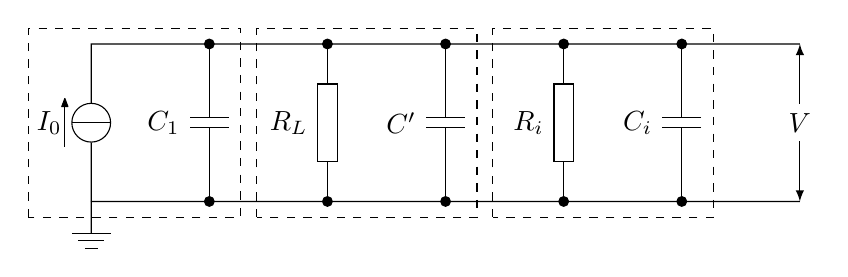
\begin{tikzpicture}[circuit ee IEC]
		\foreach \contact/\x in {1/1.5, 2/3, 3/4.5, 4/6, 5/7.5} {
			\node [contact] (up \contact) at (\x, 2) {};
			\node [contact] (dn \contact) at (\x, 0) {};
		}
		\draw (0, 0) to [current source={direction info={}, info={$I_0$}}] (0, 2) to (9, 2);
		\draw (9, 0) to (0, 0) to [ground={at end}] (0, -.5);
		\draw (dn 1) to [capacitor={info={$C_1$}}] (up 1);
		\draw (dn 2) to [resistor={info={$R_L$}}] (up 2);
		\draw (dn 3) to [capacitor={info={$C'$}}] (up 3);
		\draw (dn 4) to [resistor={info={$R_i$}}] (up 4);
		\draw (dn 5) to [capacitor={info={$C_i$}}] (up 5);
		\draw[latex-latex](9, 0)--(9, 2)node[midway, fill=white]{$V$};
		\draw[dashed](-.8, -.2)rectangle(1.9, 2.2);
		\draw[dashed](2.1, -.2)rectangle(4.9, 2.2);
		\draw[dashed](5.1, -.2)rectangle(7.9, 2.2);
	\end{tikzpicture}
	\\
	$\Downarrow$
	\\[3ex]
	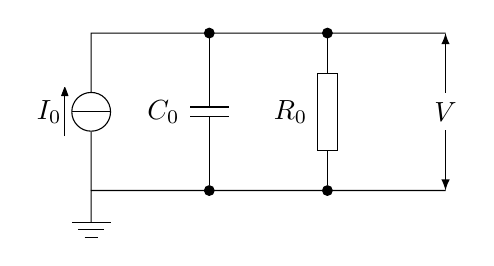
\begin{tikzpicture}[circuit ee IEC]
		\foreach \contact/\x in {1/1.5, 2/3} {
			\node [contact] (up \contact) at (\x, 2) {};
			\node [contact] (dn \contact) at (\x, 0) {};
		}
		\draw (0, 0) to [current source={direction info={}, info={$I_0$}}] (0, 2) to (4.5, 2);
		\draw (4.5, 0) to (0, 0) to [ground={at end}] (0, -.5);
		\draw (dn 1) to [capacitor={info={$C_0$}}] (up 1);
		\draw (dn 2) to [resistor={info={$R_0$}}] (up 2);
		\draw[latex-latex](4.5, 0)--(4.5, 2)node[midway, fill=white]{$V$};
	\end{tikzpicture}
	\captionof{figure}{电离室等效电路图}
\end{center}
%电流,是载流子流动的产物。其大小由(1)载流子的数量,(2)载流子单位时间扫过的电位差占极板间压差的份额决定。
%这个电流被分享了,分享者至少包括:负载电阻、测量仪器的输入电阻。
%电流流过电阻必然有压降,因此探测器极板的压差自然也会改变,这进而使得与电阻并联的极板电容、分布电容、仪器输入电容的电压也发生变化、有了充放电,因此,这些电容也就要分享电流。
%所以,整个过程就是电场驱动一定数量的载流子在极板间运动,在外电路形成了感应电流,后者流经电阻和电容后形成了电压信号。
%这个道理对于后面的闪烁探测器、半导体探测器同样适用。
\paragraph{脉冲电离室的输出电压信号}
我们虽然写出了电流的公式,也理解了它的物理图像,但并不便于直接观察它,通常,我们分析的是电压信号!

解微分方程
\[
	I_0=\frac V{R_0}+C_0\dv Vt,\implies V(t)=\frac{\e{-t/R_0C_0}}{C_0}\int_0^tI_0(\tau)\e{\tau/R_0C_0}\d\tau.
\]
定义冲击响应函数
\[
	h(t):=\frac1{C_0}\e{-t/R_0C_0},\enspace t>0.
\]
方程的解可以写成卷积的形式
\[
	V(t)=I(t)\ast h(t).
\]
\begin{definition}{弹道亏损}{ballistic deficit}
	由于在给电容充电的同时,电容就已经开始通过电阻放电,导致电容上的最大电压$V\maxi<Q/C$的现象。($Q$表示电流面积)
\end{definition}
只有在$R_0C_0\to\infty$或电流$I(t)=\delta(t)$时,才没有弹道亏损。
但这两种情况都过于理想,因此弹道亏损总是存在的!

电流持续时间越长,弹道亏损程度越严重。%因此,电流的形状会影响弹道亏损的程度。

若电流的形状是确定的,则弹道亏损的程度就是确定的,有关系$Q\propto V$,可通过$V$来分析$Q$进而分析$E\dep$。
为保证$Q\propto V$,可令
\[
	R_0C_0\gg~\text{电流持续时间},
\]
此时弹道亏损可以忽略,对应离子脉冲电离室。
\subparagraph{离子脉冲电离室}
当$R_0C_0\gg T^+$时,全部电子和正离子对输出信号都有贡献,此时为离子脉冲电离室状态。
\begin{center}
	\begin{tikzpicture}[yscale=.8]
		\coor {5.5}{4.2}tV;
		\draw[thick](0, 0)--(1, 2)--(4.2, 3.5);
		\draw[thick, domain=4.2:5]plot(\x, {3.5^((7.2-\x)/3)});
		\draw[dashed](0, 2)node[left]{$\frac{Q^-}{C_0}$}--(1, 2)--(1, 0)node[below]{$T^-$};
		\draw[dashed](0, 3.5)node[left]{$\frac{N_0e}{C_0}$}--(4.2, 3.5)--(4.2, 0)node[below]{$T^+$};
	\end{tikzpicture}
	\captionof{figure}{离子脉冲电离室的电压信号}
\end{center}
$(0,T^-)$离子电流+电子电流,$(T^-,T^+)$离子电流,$T^+$之后电容放电。在$t=T^+$时,电压信号的幅度最大,且
\begin{align}
	h:=V(T^+)=\frac{N_0e}{C_0}=\frac{e}{C_0}\frac{E\dep}W\propto E\dep.
\end{align}
因此可以测量射线的能量。

为了获得尽可能大的幅度,以抵抗后续电路的噪声,必须设法降低$C_0=C_1+C'+C_i$。

但由于要求$R_0C_0\gg T^+\sim\si{ms}$会带来问题:分辨时间大,限制了入射粒子的强度,否则会堆积;要求放大器电路频带非常宽,噪声大而非实用。
\subparagraph{电子脉冲电离室}
当$T^+\gg R_0C_0\gg T^-$时,正离子漂移的贡献可以忽略,仅有电子的贡献,此时为电子脉冲工作状态。
\begin{center}
	\begin{tikzpicture}
		\coor 43tV;
		\draw[thick](0, 0)--(1, 2);
		\draw[thick, domain=1:3.5]plot(\x, {2^(2-\x)});
		\draw[dashed](0, 2)node[left]{$\frac{Q^-}{C_0}$}--(1, 2)--(1, 0)node[below]{$T^-$};
	\end{tikzpicture}
	\captionof{figure}{电子脉冲电离室的电压信号}
\end{center}
输出电压脉冲幅度
\[
	h=V(T^-)=\frac{Q^-}{C_0}\not\propto E\dep.
\]
与初始电离位置有关($Q^-$),不能用来测量射线能量$E\dep$。

由于$R_0C_0\ll T^+\sim\si{ms}$,因此可以大大降低脉冲宽度,获得小的分辨时间。另外,减小了频带的宽度,后续电路可以较好的抑制噪声。

\subsection{圆柱形电子脉冲电离室和屏栅电离室}

\paragraph{圆柱形电子脉冲电离室}
利用圆柱形电场的特点来减少$Q^-$对入射粒子位置的依赖,达到利用\textit{电子脉冲}来测量能量的目的。

圆柱形电场距中心位置为$r$的场强
\[
	E=\frac1r\cdot\frac{V_0}{\ln(b/a)}.
\]
电离会更多地发生在电位变化趋势缓慢的大半径处,将中央作为阳极,则大部分电子在漂向阳极时扫过的电荷量接近1个$e$。
\paragraph{屏栅电离室}
正极A、负极B、栅极G\footnote{屏蔽作用,使b区的电子离子不会在阳极A上产生感应电荷。}、电源和负载电阻。
\begin{center}
	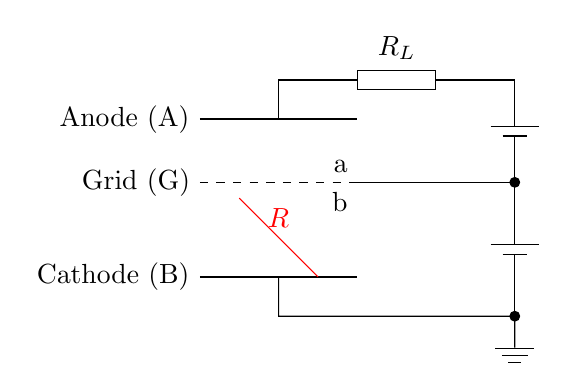
\begin{tikzpicture}[circuit ee IEC]
		\draw [thick] (-4, 2.5) node [left] {Anode (A)} -- (-2, 2.5);
		\draw [thick] (-4, .5) node [left] {Cathode (B)} -- (-2, .5);
		\draw [dashed] (-4, 1.7) node [left] {Grid (G)} -- (-2, 1.7) node [above left] {a} node [below left] {b};
		\draw (-2, 1.7) -- (0, 1.7);
		\draw (-3, .5) to (-3, 0) to (0, 0) to [ground={at end}] (0, -.5);
		\draw (-3, 2.5) to (-3, 3) to [resistor={info={$R_L$}}] (0, 3) to [battery] (0, 1.7) node [contact] {} to [battery] (0, 0) node [contact] {};
		\draw [red] (-3.5, 1.5) -- (-2.5, .5) node [midway, above] {$R$};
	\end{tikzpicture}
	\captionof{figure}{屏栅电离室结构}
\end{center}
结构要求:入射粒子将全部能量损失在b区。

入射粒子在b区产生电子离子对,电子在a区漂移时,在阳极A上形成感应电荷。

\subsection{脉冲电离室输出信号的测量}

\paragraph{入射带电粒子的数量}
测量输出脉冲数。
\paragraph{入射带电粒子的能量}
测量输出电压信号的幅度。
\paragraph{确定入射粒子间的时间关系}
测量输出电压信号的时间。

\subsection{脉冲电离室的性能}

脉冲电离室常用来测量带电粒子的能量。单能带电粒子若将全部能量都损耗在灵敏体积内,则输出电压脉冲的幅度反映了单个入射带电粒子能量的大小。
\paragraph{能量分辨率}
电离过程中的多次碰撞之间并非完全独立,离子对数目$N$服从Fano分布,当$N$很大时近似服从Gauss分布,由于
\[
	h=\frac{Ne}{C_0},
\]
电离室输出脉冲幅度$h$同样服从Gauss分布,故其半峰全宽(full width at half maxima, FWHM)
\[
	\FWHM=2\sqrt{2\ln2}\sigma_h\doteq 2.355\sigma_h.
\]

能量分辨率定义为FWHM比上均值$\avg h$
\[
	\eta:=\frac{\FWHM}{\avg h}=2.355\nu_h.
\]
又
\[
	\avg h=\frac e{C_0}\avg N,\quad\sigma_h=\frac e{C_0}\sigma_N=\frac e{C_0}\sqrt{F\avg N}.
\]
故能量分辨率为
\begin{align}
	\eta=2.355\sqrt{\frac{F}{\avg N}}=2.355\sqrt{\frac{FW_0}{E_0}}.
\end{align}
能量分辨率决定了谱仪所能达到的理论极限值,反映了谱仪对不同入射粒子能量的分辨能力。能量分辨率越好,可区分的能量差别也越小,是谱仪的主要指标之一。半导体探测器常用半宽度FWHM表征能量分辨特性
\[
	\FWHM=\eta E=2.355\sqrt{FWE}.
\]

能量分辨率的影响因素包括:统计涨落(statistical)、测量工作中条件的不稳定(drift)、探测器或电子学的随机噪声(noise)。
\[
	\FWHM^2=\FWHM_{\mathrm{stat}}^2+\FWHM_{\mathrm{drift}}^2+\FWHM_{\mathrm{noise}}^2.
\]
考虑drift因素。对于电离室谱仪,放大器输出的脉冲幅度为
\[
	h_A=A\frac{Ne}{C_0},
\]
$A$为放大倍数,故$\nu_{h_A}^2=\nu_N^2+\nu_A^2$

考虑noise因素,放大器噪声对输出幅度涨落的影响是叠加关系
\[
	h=h_1+h_2
\]
噪声的均值$\avg h_2=0$,定义信噪比$J$
\[
	J:=\frac{\avg h_1}{\sigma_{h_2}},
\]
电离室谱仪放大器输出信号的相对均方涨落$\nu_h^2$和能量分辨率$\eta$分别为
\[
	\nu_h^2=\frac F{\avg N}+\nu_A^2+\frac1{J^2},\quad \eta=2.355\sqrt{\frac F{\avg N}+\nu_A^2+\frac1{J^2}}.
\]
\paragraph{饱和特性曲线}
脉冲幅度$h$与电离室工作电压$V_0$的关系曲线。
\begin{center}
	\begin{tikzpicture}
		\coor64{V_0}h;
		\draw[thick](2, 2)parabola(0, 0);
		\draw[thick](2, 2)--(4, 2.1);
		\draw[thick](4, 2.1)parabola(5, 3)node[above]{正比区};
		\draw[dashed](0, 2)--(2, 2);
		\draw[dashed](0, 1.8)node[left]{90\%}--(1.37, 1.8)--(1.37, 0)node[below]{$V_1$};
		\draw[dashed](4, 2.1)--(4, 0)node[below]{$V_2$};
		\draw[dashed](2.25, 2)--(2.25, 0)node[below]{$V_{\mathrm{work}}$};
		\node[above right]at(0, 3){复合区};
		\node[above]at(2.75, 3){饱和区};
	\end{tikzpicture}
	\captionof{figure}{饱和特性曲线}
\end{center}
对于脉冲探测器而言,希望工作在饱和区。
在达到饱和区脉冲幅度90\% 时对应饱和电压$V_1$,正比区前是放电电压$V_2$,在二者三等分点处是饱和区的工作电压$V_{\mathrm{work}}$。

饱和区并不是水平的,虽然射线的能量沉积并没有变,但提高电压会使灵敏体积变大,复合和扩散被进一步抑制,脉冲幅度会有微小增大。
\paragraph{坪特性曲线}
电离室的计数率$n$与工作电压$V_0$的关系曲线。
\begin{center}
	\begin{tikzpicture}
		\coor64hn;
		\draw[thick, domain=0:1.5]plot(\x, {3*exp(-4*\x*\x)});
		\node[right]at(0, 3){电子学噪声};
		\draw[dashed, domain=.25:1.75]plot(\x, {2*exp(-16*(\x-1)*(\x-1))});
		\node[below]at(1, 0){复合区};
		\draw[thick, domain=-1:1, shift={(3.6, 0)}]plot(\x, {1.2*exp(-6*\x*\x)});
		\draw[thick, domain=-1:1, shift={(4, 0)}]plot(\x, {exp(-4*\x*\x)});
		\draw[thick, domain=-1:1, shift={(4.4, 0)}]plot(\x, {.8*exp(-3*\x*\x)});
		\draw[dashed](3.6, 0)node[below]{$h_1$}--(3.6, 1.5);
		\draw[dashed](4, 0)node[below]{$h_2$}--(4, 1.5);
		\draw[dashed](4.4, 0)node[below]{$h_3$}--(4.4, 1.5);
		\node at(3, -1){(a)};
	\end{tikzpicture}
	\begin{tikzpicture}
		\coor 44{V_0}n;
		\draw[dashed](2, 0)node[below]{$V_1$}--(2, 3);
		\draw[thick](3.5, 1)--(2, 1)node[midway, above]{$h_1$}parabola(1, 0);
		\draw[thick](3.5, 1.75)--(2, 1.75)node[midway, above]{$h_2$}parabola(.75, 0);
		\draw[thick](3.5, 2.5)--(2, 2.5)node[midway, above]{$h_3$}parabola(.5, 0);
		\node at(2, -1){(b)};
	\end{tikzpicture}
	\captionof{figure}{(a) $n\vs h$曲线图;(b)坪特性曲线}
\end{center}
入射粒子束流强度和入射粒子的能量保持不变,当输出脉冲幅度饱和后,计数率不再随工作电压变化;甄别阈$h_\thres$改变时,坪曲线也会改变。
\paragraph{探测效率}
绝对探测效率(absolute detection efficiency)
\[
	\varepsilon_{\mathrm{abs}}:=\frac{\text{脉冲数}}{\text{放射源放出粒子数}}.
\]
本征探测效率(intrinsic detection efficiency)
\[
	\varepsilon_{\mathrm{int}}:=\frac{\text{脉冲数}}{\text{射入灵敏体积的粒子数}}.
\]

带电粒子可能在灵敏体积内损失的能量较少,且电离过程是涨落的,信号脉冲幅度$<$甄别阈时,不能被记录。故带电射线$\varepsilon_{\mathrm{int}}\leqslant 100\%$

对中性射线,首先取决于与介质作用%产生次级带电粒子的
概率$\varepsilon=1-\e{-N\sigma D}<100\%$,然后次级带电粒子能否进入灵敏体积并沉积足够多能量。
\paragraph{时间特性}
分辨时间(死时间):能分辨开两个相继入射粒子间的最小时间间隔,由输出回路参数和放大器的时间常数决定。

时滞:入射粒子的入射时刻与输出脉冲产生的时间差。

时间分辨本领:由探测器输出脉冲来确定入射粒子入射时刻的精度。

\section{累计电离室}

入射粒子的强度$n$很大时,各个脉冲之间会发生叠加,探测器将无法再工作于脉冲模式,电离室的输出信号反映的是大量入射粒子的平均电离效应,其工作在累计或电流工作状态,此时电离室称作累计电离室或电流电离室。

%当$n$足够大,以至于在$R_0C_0$时间内的入射粒子数$\gg 1$,此时会形成直流电压信号,电流还是脉冲的;当$n$强大到在离子收集时间$T^+$内就有大量粒子入射,即使$R_0C_0=0$,$I_0(t)$也反映了大量粒子的平均电离效应,会形成直流电流信号。

假设:
\begin{compactenum}
	\item 单位时间内射入灵敏体积带电粒子数目的平均值$\avg n$不变;
	\item 带电粒子在灵敏体积内产生的离子对数目的平均值$\avg N$不变;
	\item 每个离子对产生后将立即使探测器产生一输出信号$S=f(t)$
\end{compactenum}
在时间间隔$\D\tau$内入射粒子产生的电子离子对数目$\D M=n\D\tau N$,推导得输出信号$S_t$的平均值和相对均方涨落为
\begin{align*}
	\avg S_t&=\avg n\avg N\int\zti f(\tau)\d\tau,\\
	\nu_{S_t}^2&=\frac1{\avg n}\kh{1+\frac F{\avg N}}\dvd{\int\zti f^2(\tau)\d\tau}{\kh{\int\zti f(\tau)\d\tau}^2}.
\end{align*}
可以看出,相对均方涨落$\nu_{S_t}^2$主要决定于入射粒子数$\D n$的涨落,离子对数$N$的涨落影响很小。
\paragraph{电流信号}用宽度为$T$的矩形脉冲近似代表一对离子所产生的电流信号
\[
	f(t)=\begin{cases}
		\frac eT,&t<T\\
		0,&t>T
	\end{cases}
\]
则电流信号的平均值和相对涨落为
\begin{align}
	\avg I&=\avg n\avg Ne,\\
	\nu_I^2&=\frac1{\avg n}\kh{1+\frac F{\avg N}}\frac1T\doteq\frac1{\avg nT}.
\end{align}
\paragraph{电压信号}
当$R_L\neq 0$时,在输出端输出一直流电压信号,一个离子对漂移在输出回路所产生的电压信号近似为一指数衰减信号:
\[
	f(t)=\frac e{C_0}\e{-t/R_0C_0}.
\]
则电压信号的平均值和相对涨落为
\begin{align}
	\avg V&=\avg n\avg NeR_0=\avg IR_0,\\
	\nu_V^2&=\frac1{\avg n}\kh{1+\frac F{\avg N}}\frac1{2R_0C_0}\doteq\frac1{2\avg nR_0C_0}.
\end{align}
要求输出电流或电压信号的相对均方涨落$\ll 1$,则
\begin{compactenum}
	\item 
	当入射粒子平均时间间隔$\ll$输出回路的时间常数:
	\[
		\frac1{2\avg n}\ll R_0C_0
	\]
	时,可视为直流电压信号;
	\item 
	当入射粒子平均时间间隔$\ll$电流脉冲宽度:
	\[
		\frac1{\avg n}\ll T
	\]
	时,可视为直流电流信号。
\end{compactenum}
\paragraph{小结}
\begin{compactenum}
	\item 脉冲电离室与累计电离室仅是电离室的两种工作状态;电离室结构并无本质差别。
	\item 入射粒子流的强度$n$及输出回路的时间常数$R_0C_0$、电流持续时间$T$决定了它工作在什么状态。
\end{compactenum}
\paragraph{累计电离室的主要性能}
饱和特性:同脉冲,工作于饱和区。

灵敏度($\si{A/cm^2.s}$)
\[
	\eta:=\frac{\text{输出电流(电压)幅度}}{\text{入射粒子流的强度}}.
\]
影响因素:电离室的结构、气体压力和组分、入射粒子的类型和能量等。

线性范围:输出信号幅度与入射粒子流强度保持线性关系的辐射强度范围。对应饱和区范围。当入射粒子流强度增大时,饱和电压将提高,会超过工作电压。

响应时间:入射粒子流强度发生变化时,输出信号的变化规律。电流主要由离子收集时间$T^+$决定,电压主要由时间常数$R_0C_0$决定。

能量响应:灵敏度随入射粒子能量而变化的关系。一般情况下,希望无能量响应。
\paragraph{累计电离室的应用}
累计电离室的应用比脉冲电离室更为广泛,特别是充入高压工作气体的
累计电离室,灵敏度高、性能稳定可靠、工作寿命长。

由于具有十分良好的承受恶劣工作环境影响的能力,所以在工业上可应
用于核辐射密度计、厚度计、料位计、水分计、核子秤等。
累计电离室还可应用于剂量测量、反应堆监测等方面。

\section{正比计数器}

脉冲电离室测量低能粒子(如$<\SI{100}{keV}$的X射线)时,放大器噪声使信噪比很小,测量难于进行。正比计数器能在探测器内部对电离信号进行放大,提高信噪比,就可以对低能粒子进行测量了。

正比计数器是一种非自持放电的气体电离探测器。利用碰撞电离将入射粒子直接产生的电离效应进行放大,使输出信号幅度比脉冲电离室显著增大。

要求:放大、均匀(位置一致)、线性(能量一致)。

\subsection{正比计数器的工作原理}

\paragraph{正比计数器的结构特点}
利用圆柱形电场的特点:\textit{在中央丝极附近会产生小范围的强电场区域}。
%强电场,以满足实现碰撞电离的要求()。
%一般采用非均匀电场实现,以圆柱型为主。

正比计数器的起始电压(阈压) $V_{\mathrm T}$,
\[
	V_{\mathrm T}=a\ln(b/a)E_{\mathrm T}.
\]
若工作电压$V_0<V_\mathrm T$,正比计数器仍是电离室;
$V_0>V_\mathrm T$时处于正比区,仅在$a\vs r_0$间发生碰撞电离。
\begin{example}{}{}
	$\SI{1}{atm}$下,电子在气体中的自由程$\sim\SIrange{e-4}{e-3}{cm}$,气体的电离电位$\sim\SI{20}{eV}$,电离所需的相应场强$E_\mathrm T=\SI{e4}{V/m}$。

	$a=\SI{80}{\micro m},b=\SI{1}{cm},V_0=\SI{4000}{V}$,计算得
	\[
		V_\mathrm T=\SI{386}{V},\quad r_0=\SI{410}{\micro m}.
	\]
	%碰撞电离
	电子漂移过的电位差
	\[
		V_\elc<\frac{\ln(r_0/a)}{\ln(b/a)}V_0=0.3384V_0,
	\]
	%碰撞电离
	离子漂移过的电位差
	\[
		V_\i>\frac{\ln(b/r_0)}{\ln(b/a)}V_0=0.6616V_0.
	\]
	故正比计数器输出电荷信号\textit{主要由正离子漂移贡献}。
\end{example}
$r_0$与$a$是同一数量级,故%入射粒子在$r_0$内产生初始电离的可能性很小,
$<r_0$处的初始电离很少。不同位置的初始电离都经受同样的气体放大过程。%故所有同一个气体放大倍数

正比计数器虽然是以离子电流为主,但它的离子电流是确定的、有快的成分,因此不必用大的$R_0C_0$
\paragraph{碰撞电离与气体放大}
电子到达距丝极一定距离$r_0$之后,通过碰撞电离过程,电子的数目不断增殖,这个过程称为气体放大过程,又称电子雪崩(electron avalanche)。定义气体放大倍数
\begin{align}
	A:=\frac{n(a)}{n(r_0)}.
\end{align}
放大倍数与Townsend系数
\[
	\alpha:=\frac1n\dv nx.
\]
有关,$\alpha$是气体类型和约化场强的函数。
\newpage
均匀电场$A=\e{\alpha\D x}$与初始位置有关,而圆柱形电场
\[
	A=\exp\biggkh{-\int_{r_0}^a\alpha\d r}.
\]
与初始电离位置无关。

$\alpha=N\sigma$,碰撞电离截面$\sigma$正比于电子的动能,故当$V_0\gg V_\mathrm T$时,
\[
	\ln A\propto V_0
\]
\paragraph{气体放大过程中的光子作用}
在电子与气体分子的碰撞中,不仅能产生碰撞电离,同时也能产生碰撞激发,退激发出的紫外光子能量一般大于阴极材料的表面逸出功,可在阴极(或其它气体分子)打出次电子,次电子在电场加速下也可发生碰撞电离,称为\textbf{光子反馈}。

定义每个到达阳极的电子通过光子反馈又在阴极打出一个次电子的概率为光子反馈概率$\gamma$,光子反馈使得总放大倍数增加为
\[
	A\tot=A+\gamma A^2+\gamma^2A^3+\cdots=\frac A{1-\gamma A}.
\]

\begin{compactitem}
	\item 光子反馈时间(\si{ns}) $\ll$电子漂移时间(\si{\micro s}),对信号形成而言可认为是同时事件。
	\item 加入少量多原子分子气体M (CO$_2$, CH$_4$)的作用:M可以强烈吸收紫外光子而处于激发态M$^*$,M$^\ast$不再发出光子而是分解为几个小分子(超前离解),这样可以阻止紫外光子打到阴极而减小光子反馈,使$\ln A\propto V_0$曲线的变化平缓,使发生自持放电的电压更高,以获得更大的正比工作区间。
\end{compactitem}
\paragraph{气体放大过程中正离子的作用}
空间电荷效应(space charge effect):在电子漂移、碰撞电离等过程中,漂移速度慢的正离子可认为基本没动,在阳极丝附近形成空
间电荷,使阳极丝附近的电场强度变弱,影响电子雪崩过程。%影响空间电场、进而影响倍增过程。

离子反馈:正离子漂移到达阴极,在与阴极表面的感应电荷中和时有一定概率产生次电子,发生新的电子雪崩过程。可以通过加入少量多原子分子气体阻断。

正比计数器雪崩不是很强烈,一个地方发生的雪崩并不妨碍其他地方能不能够发生雪崩。

\subsection{正比计数器的输出信号}

\paragraph{离子电流}假定:
\begin{compactenum}
	\item $A\gg 1$:忽略初始电离的载流子对输出信号的贡献。
	\item $r_0$很小:电子的阴极感应电荷很小$\to$忽略电子对输出信号的贡献。
	\item 全部输出信号为雪崩后正离子由阳极表面向阴极漂移在外回路流过的感应电荷。
\end{compactenum}
则
\begin{gather*}
	I=A\frac{Ne}{V_0}\bm E\cdot\bm u^+,\\
	u^+=\mu^+\frac EP,\implies\dv rt=\frac{\mu^+}P\frac{V_0}{r\ln(b/a)}.
\end{gather*}
得到
\[
	I=\frac{ANe}{2\ln(b/a)}\frac1{t+\tau},\quad\tau:=\frac{a^2P\ln(b/a)}{2V_0\mu^+}=\SI{15.1}{ns}.
\]
故电流$I$随时间$t$下降地很快!
\begin{align}
	I\propto\frac1{t+\tau}.
\end{align}
离子电流虽然持续时间很长,但很早就扫过了大部分电荷

无论射线在哪里发生初始电离,正比计数器输出电流的形状总是确定的,则电压信号的弹道亏损程度总是确定的。
电流面积受两个因素影响:初始电离的载流子数目$N_0\propto E\dep$;倍增系数$A$反映雪崩的剧烈程度,对一个确定的探测器来说,$A$的期望值仅由工作电压$V_0$决定。
因此正比计数器输出电压信号的幅度$h\propto E\dep$,这是很重要的特点。
\paragraph{电压信号}
\[
	V_0=\frac{ANe}{2C_0\ln(b/a)}\e{-t/R_0C_0}\int_0^t\e{t'/R_0C_0}\frac{\d t'}{t'+\tau}.
\]
电压脉冲信号与粒子入射位置无关,$R_0C_0$的选取虽会影响电压幅度,但$h\propto N$仍成立。

由于离子电流在早期即\textit{扫过了大部分电荷},因此可以在不过分减小信号幅度的情况下,减小$R_0C_0$以实现高的计数率。

\subsection{正比计数器的性能}

\paragraph{输出脉冲幅度与能量分辨率}
输出脉冲幅度$h\sim ANe/C_0$是一个二级串级型随机变量,其相对涨落
\[
	\nu_h^2=\nu_N^2+\frac1{\avg N}\nu_M^2=\frac1{\avg N}\kh{F+\nu_M^2}.
\]
实验表明$\nu_M^2\doteq 0.68$,故能量分辨率
\begin{align}
	\eta=2.355\sqrt{\frac{F+0.68}{\avg N}}.
\end{align}
影响正比计数器能量分辨率的其它因素:阳极丝的均匀性、负电性气体的存在、末端效应和室壁效应、电子学系统的影响。
\[
	\nu_{h_A}^2=\frac F{\avg N}+\frac1{J^2}+\nu_A^2=\frac F{\avg N}+\frac{\nu_M^2}{\avg N}-\kh{\frac{C_0\sigma_{h_2}}{ANe}}^2+\nu_A^2.
\]
在满足信噪比的前提下,可用小的倍增系数,有利于:减少非线性、获得好能量分辨率。
\paragraph{探测效率和坪特性}
分立$\vs$连续,见讲义
\paragraph{分辨时间$\tau$和计数率修正}
分辨时间$\tau$:主要由输出脉冲的宽度决定。%脉冲越宽,死时间越大。在$\tau$内再产生的脉冲不会被记录,从而会造成计数的损失,为此必须考虑计数率的修正。

任何一个信号,只有当其前面$\tau$时间内无信号时,才能被计数。考虑平均计数率为$m$,则$\tau$内无信号的概率为$\e{-m\tau}$,因此,实际测量到的计数率$n=m\e{-m\tau}$,当$m\tau\ll 1$时,
\begin{align}
	n=m\e{-m\tau}\doteq m(1-m\tau),\implies m\doteq\frac n{1-n\tau}.
\end{align}
第二个射入探测器的射线能否被探测器响应要看探测器测量它的条件是否具备。就正比计数器来说,有气体可初始电离形成自由电子,有电场可雪崩,%只要不恰巧在上个射线正离子未漂走的雪崩处,
则第二个射线肯定是可以被探测器响应的。%同理,第三个、第四个……也是可以被响应的。

但是电路只有一个,这些被响应射线的输出信号可能就由于其间隔小于分辨时间而不得不叠加为一个电信号,这就是计数率损失的来源。
\paragraph{时滞与时间分辨本领}
时滞(\si{\micro s}):初始电子由产生处漂移到阳极附近所需的时间。

时间分辨本领(\si{\micro s}):正比计数器对时间的测量精度。由于初始电子产生位置的随机性,因此时滞也具有随机性,从而限制了时间分辨本领。

\subsection{正比计数器的应用}

能量测量——正比谱仪

正比计数器在强度测量方面的应用

单丝位置灵敏正比计数器

多丝正比室

GEM探测器

\section{G-M计数管}

G-M计数管是由Geiger和Müller于1928年发明的一种利用自持放电来进行射线探测的气体电离探测器,它也许是最著名的射线探测器。

G-M管的优点:制造简单、价格便宜、使用方便、灵敏度高、输出电荷量大($10^8e$);缺点:死时间长、仅能用于计数。
%✓

\subsection{非自熄G-M管的工作机制}

在正比计数器中,光子反馈和正离子反馈的作用极微弱,因此,经一次雪崩以后增殖过程即行终止,且雪崩只限于局部的区域,对一个初始电子仅展宽$\SI{200}{\micro m}$左右;但在G-M计数管中,光子反馈和离子反馈就成为重要的过程。

由于光子反馈过程的存在,气体放大倍数为
\[
	A\tot=\frac A{1-A\gamma},
\]
通常条件下光子反馈概率为$\gamma\sim 10^{-5}$,若$A\sim 10^5$,则$A\tot\to\infty$

G-M管的自持放电过程可以分解为下列环节:
\begin{compactenum}
	\item 初始电离及碰撞电离过程:电子加速发生碰撞电离形成电子潮(雪崩)。
	\item 放电传播:Ar$^*$放出的紫外光子打到阴极上并打出次电子(光子反馈)。
	
	一处点火,全丝放电:气体放电迅速遍及整个管子。
	
	电子很快被阳极收集,形成电子电流;正离子包围整个阳极丝,并逐步加厚形成正离子鞘。由于正离子鞘的形成,使阳极丝附近的电场减弱,使放电终止。
	\item 正离子鞘向阴极漂移,形成离子电流,是形成输出脉冲的主要贡献。
	\item $\sim\SI{100}{\micro s}$后正离子在阴极表面发生电荷中和,形成\textbf{离子反馈}:
	\[
		\nuc{Ar}^++\elc^-\to\nuc{Ar}^\ast\overset{\star}\semilongrightarrow\elc^-\overset{\text{加速}}\semilongrightarrow\nuc{Ar}^++\nuc{Ar}^\ast+\elc^-\overset{\text{加速}}\semilongrightarrow\cdots
	\]
	$\star$:Ar$^\ast$退激发射光子打到阴极或Ar$^\ast$直接到达阴极。

	它们发生在第一次正离子漂移快结束时;阴极产生的电子向阳极漂移又引起新的雪崩,形成第二个脉冲;如此周而复始,形成了自持放电,所以被称作非自熄G-M计数管。
\end{compactenum}
\paragraph{如何实现自熄?}雪崩的两个条件:电场和电子。

外因自熄(external quenching):改变工作高压(影响电场)。在脉冲产生后,降低工作高压,使倍增条件不具备,持续时间应该包括:
\begin{compactitem}
	\item 离子由正离子鞘漂移到阴极的时间:$\sim\SI{100}{\micro s}$
	\item 阴极产生的自由电子运动到阳极的时间:$\sim\si{\micro s}$
\end{compactitem}
可以在外电路选用大电阻($R\sim\SI{e8}{\ohm}$),$R_0C_0\sim\si{ms}$,满足自熄要求,但也需要$\sim\si{ms}$来使阳极恢复到正常工作状态,因此计数率低。

内因自熄(internal quenching):增加猝熄气体(影响电子),比如有机自熄G-M管、卤素自熄G-M管。

\subsectionstar{有机自熄管的工作机制}

有机自熄管是在工作气体中加入少量有机气体M (多原子分子气体,又称猝熄气体)具有自熄能力的G-M管。例如,90\% Ar + 10\% C$_2$H$_5$OH。

阻断光子反馈,阻断离子反馈……

工作电压较高、寿命较短。

\subsectionstar{卤素自熄管的工作机制}

Ne为主要工作气体,并在其中加入微量卤素气体(如1\% Br)

自动猝熄、较低阈压、寿命较长、放电区域较大、卤素为负电性气体(影响卤素计数管的特性,尤其是坪特性曲线。有机管的坪特性好些)

\subsection{自熄G-M管的输出信号}

自熄G-M计数管输出脉冲形状与正比计数管无明显区别。和正比计数器一样,输出脉冲由两个部分组成:
\begin{compactenum}
	\item 电子收集、正离子漂移初期的快上升部分
	\item 正离子漂移期间的缓慢上升部分
\end{compactenum}
\begin{center}
	\captionof{table}{正比计数器与G-M管比较}
	\begin{tabular}{ccc}
		\toprule
		&正比计数器&G-M管\\
		\midrule
		输出信号的幅度&$\propto E\dep$&与能量无关\\
		用途&测能谱、计数&只能用于计数\\
		\bottomrule
	\end{tabular}
\end{center}

\subsection{自熄G-M管的性能}

G-M管的性能由以下因素决定:计数管的阳极丝半径$a$、阴极半径$b$、工作气体的组成与压力。

主要性能包括:坪特性曲线、探测效率、时间特性
\paragraph{坪特性曲线}计数率与工作电压的关系……

坪斜的成因:随工作电压的增高,
\begin{compactenum}
	\item 正离子鞘电荷量增加,猝熄不完善的可能性增加
	\item 负电性气体的电子释放概率增加
	\item 灵敏体积增大
	\item 结构的尖端放电增加
\end{compactenum}
\paragraph{探测效率}
对用于带电粒子探测的钟罩型G-M管,只要入射粒子进入灵敏体
积,其探测效率可接近100\%。

对用于探测$\gamma$射线的圆柱型G-M管,仅当次电子进入灵敏体积才能引起计数,其探测效率仅$\sim 1\%$。
\paragraph{时间特性}
\begin{compactitem}
	\item \textbf{失效(死)时间}$t_\mathrm d\sim\SI{100}{\micro s}$:随正离子鞘向阴极漂移,使电场屏蔽逐渐减弱、电子又能在阳极附近发生雪崩的时间。
	\item \textbf{时滞}:在气体中生成第一个离子对的时间与第一个雪崩的时间存在延迟,且延迟时间与第一个离子对生成的位置有关。其差别$\SIrange{0.1}{0.4}{\micro s}$,会导致这一量级时间测量的不准确性。
	\item \textbf{时间分辨本领}$\sim\si{\micro s}$,采取特殊措施后可$\sim\SI{0.1}{\micro s}$。
	\item \textbf{复原时间}$t_\mathrm e\sim\SI{100}{\micro s}$:从上一个事件开始,输出脉冲幅度恢复到正常的时间。
	\item \textbf{分辨时间}$t_\mathrm f\sim\SI{100}{\micro s}$:从0到下一个脉冲超过甄别阈的时间,与甄别阈的大小有关。\footnote{一般死时间同分辨时间,但G-M管的死时间特指失效时间,是分辨时间的一部分。}
\end{compactitem}
G-M管中,由于正离子鞘覆盖了整个阳极丝,在第一个粒子引起的死时间内,不能产生新的雪崩,死时间因此不再扩展。\footnote{G-M管大概是死时间唯一不可扩展的探测器类型了,本课程的其它探测器(电离室、正比计数器、闪烁探测器、半导体)的死时间都是可扩展的,其共同的机制就是:\textit{一个射线的入射不会使探测器失能、从而导致无法响应下一个时间上邻近的入射射线。}}

真事件的计数率为$m$,探测器死时间为$\tau$,记录到的计数率为$n$,则有
\begin{align}
	\frac1m=\frac1n-\tau.
\end{align}
\paragraph{寿命}计数寿命:有机管$\sim 10^8$次计数,卤素管$\sim 10^9$次计数;

搁置寿命:卤素管中的卤素较活泼,寿命较短。有机管可保证长达几年的搁置寿命。
\paragraph{输出回路对计数管特性的影响}
在G-M管中,尤其是对卤素管,其放电区域较大,电子漂移对输出信号的贡献比正比计数器要大,对放电终止有影响。

尽可能减小分布电容有利于提高输出脉冲幅度,对放电终止也起到积极作用。

\subsectionstar{自熄G-M管的结构与典型应用}

G-M管主要有:
\begin{compactenum}
	\item 圆柱型:主要用于$\gamma$射线测量
	\item 钟罩型:由于有入射窗,主要用于$\alpha,\beta$射线的测量
\end{compactenum}
\newpage
\paragraph{气体探测器的问题?}气体探测器的能量分辨率
\[
	\eta=2.355\nu_h=2.355\sqrt{\frac{F+0.68}{\avg N}}
\]
是不错的,对重带电粒子和低能光子的测量是出色的。

但它不能测量高能光子,原因:
\begin{compactenum}
	\item 与MeV光子的反应概率$1-\e{-N\sigma D}$
	\item 对MeV电子能量的沉积能力
\end{compactenum}
我们下面讨论闪烁体探测器。

